\chapter{Grundlagen und theoretischer Rahmen}
\label{StandDerForschung}

\section{Datenintegration und -analyse}
Relevante Quellen:
\begin{itemize}
    \item IT-Management\cite{tiemeyer2023}
    \item Data Engineering \cite{reis2023}
    \item BPM Übersicht \cite{weske2019}
    \item 
    \item Speziellere Werke zum Thema
\end{itemize}


Joe Reis und Matt Hously gehen in einem Grundlagenwerk zum Thema Data Engineering auf grundsätzlich relevante Phasen, Aspekte und Fragestellungen anhand des "Data Engineering Lifecycles" von der Datengenerierung über Ingestion, Transformation, Speicherung und Bereistellung bis hin zur Analyse ein. \cite{reis2023} 


\begin{itemize}
\item Hier wird auf Literatur im Bereich Datenintegration und Analyse eingegangen
\item Das Kapitel gibt einen groben Überblick welche Aspekte basierend auf Literatur im Bereich Datenintegration und Analyse beachtet werden müssen
\item Wichtigstes Grundlagenwerk ist das „Handbuch Data Engineering: Robuste Datensysteme planen und erstellen“ von Joe Reis und Matt Housley, welches das Forschungsgebiet "Data Engineering" umfassend beschreibt, Grundbegriffe definiert und relevante Konzepte behandelt und auf weitere relevante Quellen verweist.
\end{itemize}

Der wesentliche Teil der Arbeit lässt sich dem Themengebiet \textit{Data Engineering} zuordnen. Das wohl bekannteste Grundlagenwerk in diesem Themengebiet ist das Buch \textit{Fundamentals of Data Engineering: Plan and Build Robust Data Systems} von Joe Reis und Matt Housley, die unterschiedliche Definitionen des Begriffs \textit{Data Engineering} vorstellen und ihn zusammenfassend wie folgt definieren (in Deutsche übersetzt) \cite{reis2023}:

\begin{quote}
    \textit{Data Engineering ist die Entwicklung, Implementierung und Wartung von Systemen und Prozessen, die Rohdaten aufnehmen und hochwertige, konsistente Informationen erzeugen, die nachgelagerte Anwendungsfälle wie Analysen und Machine Learning unterstützen. Data Engineering ist die Schnittstelle zwischen Sicherheit, Datenmanagement, DataOps, Datenarchitektur, Orchestrierung und Softwareentwicklung.}
\end{quote}

Reis und Housley etablierten mit den \textit{Data Management Lifecycle} (siehe \autoref{fig:Data Engineering Lifecycle}) außerdem eine systematische, praxisorientierte und mittlerweile verbreitete Abgrenzung der Themenbereiche des \textit{Data Engineerings}. 

\begin{figure}
    \centering
    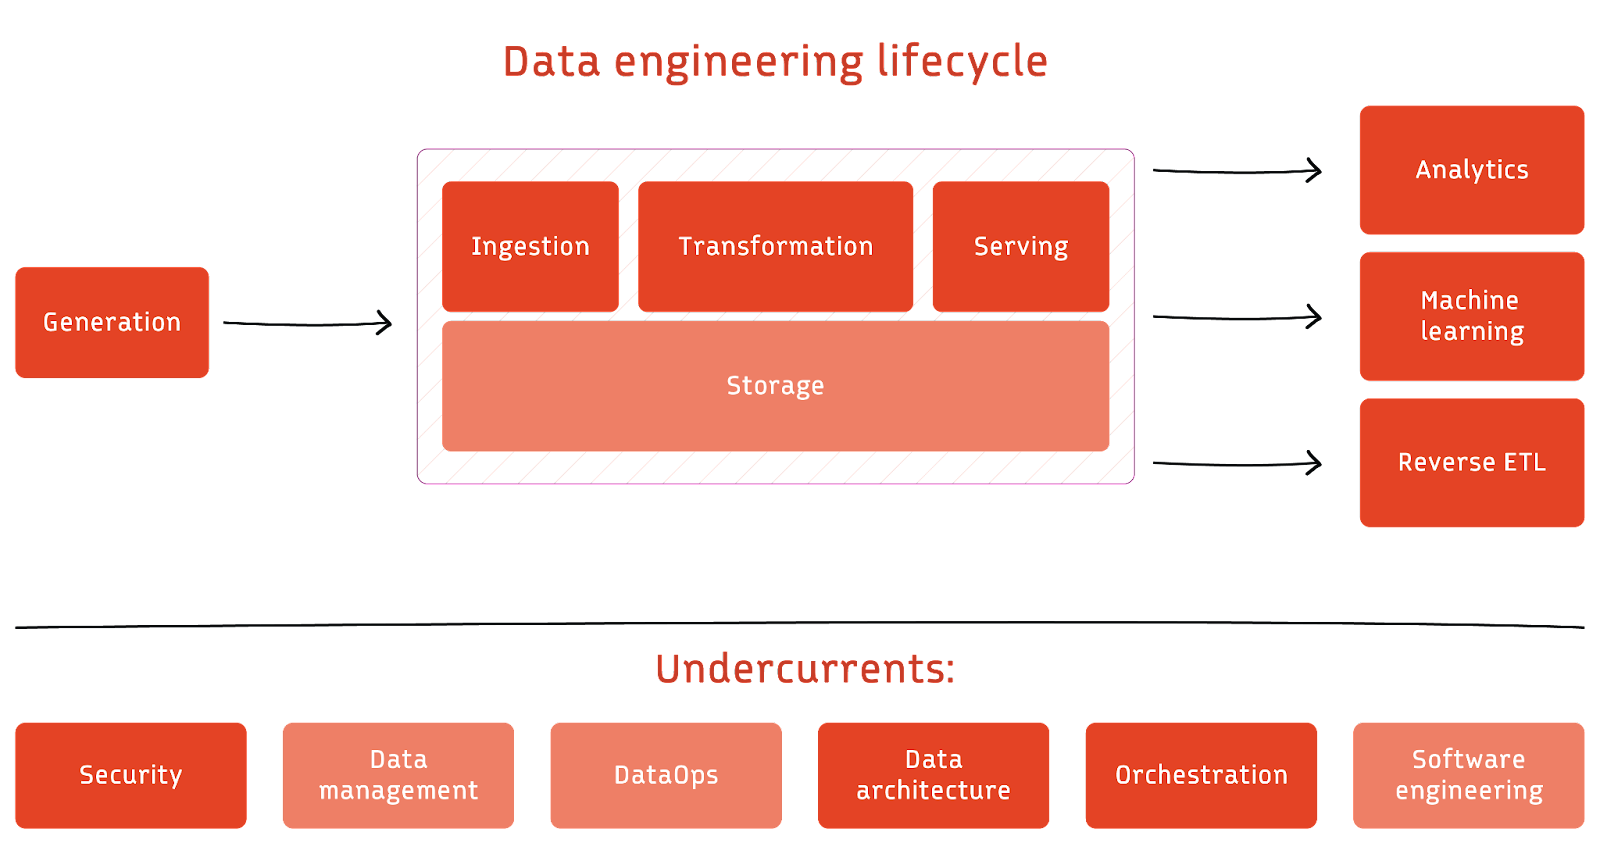
\includegraphics[width=1\linewidth]{Grafiken/Data Engineering Lifecycle.png}
    \caption{Data Engineering Lifecycle}
    \label{fig:Data Engineering Lifecycle}
\end{figure}

\subsection{Grundlagen zu Materialien}

\section{Systemübersicht - Die X4 BPMS und datengetriebene Geschäftsmodelle}
\label{Systemübersicht}

\subsection{Allgemeine Grundlagen der X4 BPMS}
\subsection{Daten und Schnittstellen der X4 BPMS}
\subsection{Analyse der Anwendungsfälle und Anforderungen an die X4 BPMS}

\section{Bestehende Ansätze und Technologien}
\subsection{Allgemeine Konzepte und Technologien}
OLAP vs. OLTP \cite{kleppmann2017} S. 91 in "Designing Data Intensive Applications" 

\subsection{Vorstellung existierenderLösungen und Produkte im Kontext der Geschäftsprozessüberwachung}
\subsection{Zusammenfassung der Ergebnisse}

